\documentclass[12pt]{article}
\usepackage[a4paper,bindingoffset=0.2in,%
            left=0.5in,right=0.5in,top=0.5in,bottom=1in,%
            footskip=.25in]{geometry}
\usepackage{hyperref}
\usepackage{amsmath}
\usepackage{graphicx}


\begin{document}

%\begin{titlepage}
   \begin{center}
       \vspace*{1cm}
 
       \textbf{FAI Draft Report}
       \vspace{1cm}
       
       \textbf{Mason Leon and Naveen Kumar Chiluka}
        \vspace{1cm}
%        \vfill
       CS 5100 \\
	Foundations of Artificial Intelligence \\
	Dr. Lawson L.S. Wong \\
	Fall 2019

 
       \vspace{0.8cm}

       Khoury College of Computer Sciences\\
       Northeastern University\\
       Boston,MA\\
        
   \end{center}
%\end{titlepage}
%\maketitle
 
\tableofcontents

\clearpage
\section{Introduction}
\subsection{Problem}
Chess has been a challenging game to be solved for many years in the field of AI. It's been tough due to the fact that its state space is too large (around $10^{50}$ states) and it would be computationally impossible to play a game without any approximation. In order to build a good AI agent there need to be heuristics for every move to finish the game.

\subsection{Motivation} The game provides a good opportunity to learn about designing evaluation functions based on the features of the game. It also helps us in understanding the nuances of the game through an AI lens and apply the concepts learned from  the course to another game.


\subsection{Objective}
To build an AI Chess Agent using Minimax Algorithm, Alpha-beta pruning along with a reasonable evaluation function.

\subsection{Problem formulation}
\begin{itemize}
\item State space: All the valid board configurations.
\item Action space: All the valid moves of the pieces.
\item Goal state: The state where the AI agent wins, loses or draws.
\item Utility or Evaluation function: Heuristic based on key features.
\end{itemize}	

\subsection{Ideal Outcome}Build an AI agent using different evaluation functions and analyze the performances of each of these cases.


\section{Approach}
\subsection{Environment}
We initially planned to use Javascript environment for the project but as both of us are
completely new to front-end development it was taking longer than expected to comfort-
ably code in JS.As we researched implementation of our algorithms, we discovered python-chess, a pure
Python chess library with move generation, move validation and support for common chess
formats. This project was exciting for us because it allowed us to work on the project in
a language we were comfortable with as well as utilize data science tools such as Jupyter
Notebooks, Google Colab, and Pandas for running, benchmarking, and performing sta-
tistical analysis of our results. Additionally, this library allows for integration of popular
chess engines for the purpose of testing our algorithm against another intelligent chess
player agent.In reading the python-chess documentation, we were directed to a Jupyter Notebook
from Dr. Douglas Blank' CS371: Introduction to Cognitive Science course at Bryn Mawr
College. In this starter code we learned about the library's basic Board, Game, and
Piece data structures and state representation of the library. We adapted the examples
of a random agent, a human agent, naive agent, and their respective evaluation functions
for our own project and have set up the chess game environment.
\subsection{Agents}
\subsubsection{Random Agent}
We have started with a Random Evaluation function which picks a random move from the available legal moves. As expected, the results were random. 
\subsubsection{Naive Agent}
So, after doing some research on the chess evaluation strategies, we discovered Material scores for the board. Material score is a heuristic that computes the utility of a particular state of the board based on the available pieces and the corresponding weights.
 $$
Material Score =\sum_{\forall \: i \: in \: pieces}^{} w_p(i)*(nW(i)-nB(i))$$
where \\
 i = piece type \\
nW(i) = number of white pieces of type i \\
nB(i) = number of black pieces of type i\\

\noindent Based on the reasoning provided on this wiki  \href{https://www.chessprogramming.org/Simplified_Evaluation_Function}{Chess Programming Wiki}
we decided on the following values for the weights for our material score heuristic: \\
Pawn = 100 \\
Knight = 320 \\
Bishop = 330 \\
Rook = 500 \\
Queen = 900 \\

\subsubsection{Improved Naive Agent}
We found that the Material Score heuristic is of not much help since its effect is seen only when there is a capture. For that to happen the agent's pieces should be in positions where it's possible to capture the opponent's pieces. We observed that the Naive agent was resulting in draws when pitted against a Random Agent more often than not. So, we imparted a little more intelligence to it by adding a couple of additional features like:
\begin{itemize}
\item score would be increased by 50 if the move results in a capture.
\item score would be increased by 9999 if the move results in a checkmate.
\item score would be decreased by 500  if the move results in a check to the current player.
\item score would be increased by 900 if the move results in a check to the opponent player.
\item score starts from a random seed unlike in the previous evaluation where it started from zero.
\end{itemize}
Adding these features, showed some positive results in the performance of the agent and resulting
in wins most of the time against the Random Agent.

\subsubsection{Advanced Agent}
The Improved Naive Agent was a reasonable player and picked better moves over Naive agent but
it would still end up picking sub-optimal moves since the features are not enough. In search of a
better heuristic we found Piece-Square tables. The tables can be thought of as Reward functions for
each of type of piece. There would be positive and negative rewards for each square of the board
for every type of piece. So, we created an Advanced Agent which relies on both Material Score and
Piece-Square Tables. Please refer to section 6 for the actual tables used in the project. This agent
performed far better than its predecessor against the Random Agent.
To illustrate the concept of Piece-Square Tables, consider the following Pawn Table:
In the below table, the top rows represent the white side while the bottom two rows represent the
black side and the table is used for white pieces.The positive values are rewards for the agent if a
pawn is moved to that square while negative values are penalties for moving to that square. This
can dictate the movement of pawns in the intended directions. As per the table, the central pawns
are levied with heavy penalty if they don't move forward and make room for minor pieces and queen.
All the pawns are encouraged to make it to the other end so that they can be promoted to more
powerful pieces.
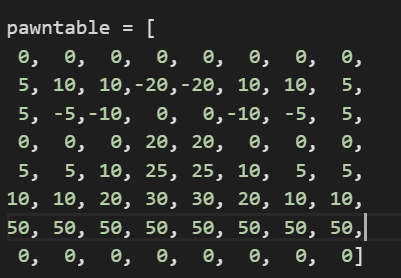
\includegraphics[scale=1]{./images/pawntable.PNG}
\begin{itemize}
\item Similarly, the Knights are encouraged to go to the center as they have the highest degree of
freedom there.
\item  The Bishops are discouraged from moving to corners and borders. They are encouraged to
move to the center as they serve better purpose there.
\item  The Rooks are discouraged from moving to the edges as they are underutilized there. They
are incentivized either to go to the opponent's side or not-penalized for being in the central
square.
\end{itemize}
\subsubsection{Mini-max Agent}
Just the two heuristics were not enough for our agent to perform well against other intelligent chess agents. The agent needed to look ahead into the future and predict the moves of the opponent and then make decisions. So, we implemented a mini-max search algorithm along with the Material Score and Piece-Square Table heuristics. This was by far the best agent we have created so far. 

\subsubsection{Mini-max-Alpha-Beta Agent}
Although the Mini-max Agent was faring well with other agents, it was taking too long to make a move when the depth of the search was more than 3. So to tackle this problem, we improved the Mini-max algorithm by incorporating the Alpha-Beta pruning technique. This technique will help the agent avoid expanding unnecessary moves. 



\subsection{Tools/Libraries}
\begin{table}[h!]
  \begin{center}
    \label{tab:table1}
    \begin{tabular}{l|c} 
      \textbf{Development Environment} & \textbf{Libraries} \\
      \hline
      Jupyter,Pycharm & python-chess\\
      Anaconda & stockfish\\
      Pandas & Syzygy API\\
    \end{tabular}
  \end{center}
\end{table}
\section{Results}
Mini-max-Alpha-Beta Agent is now improved due to the Advanced Evaluation Function in the following ways:
\begin{itemize}
\item Number of moves required to win
\item Reduced overall losses ( leading either to a win or a draw )
\end{itemize}


\section{Problems Faced}
\begin{itemize}
\item Analyzing the game and deciding on the features was tougher than we thought.
\item Due to the space and time complexity of the game, it was difficult to debug the game as every game would take long time to run till the end depending on the evaluation function. We could use PyCharm for debugging but it was not a feasible option for us due to the limitations of our local machines. So, our only option was to run on google co-lab servers but the debugging features of the Jupyter notebook were limited and not very helpful.
\item We encountered difficulties while integrating our agent with another trained, intelligent chess agent like Stockfish. The problem was the Jupyter support with File IO. We had Permission errors while uploading the executable file of the Stockfish engine. We are still in the process of fixing this issue.
\item There were confusions over obscure chess rules automatically built into the library resulting in draws.
\end{itemize}
\section{Next steps}
\begin{itemize}
\item We are currently working on finishing migrating utility and API functions to an external Python file to ease Jupyter notebook debugging.
\item We intend to integrate a trained, external agent (stockfish) with our program to see our agents fare with that.
\item We plan to utilize an API with endgame statistics to compare the performance of our agents against millions of others at same state and use the data to determine if our heuristics are improving performance.

\end{itemize}


\section{References}
\label{References}
\begin{itemize}
\item Fiekas, Niklas et al. python-chess: a pure Python chess library. Github.
\url{https://github.com/niklasf/python-chess}

\item Fiekas, Niklas et al. python-chess: a pure Python chess library. ReadtheDocs.
\url{https://python-chess.readthedocs.io/en/latest/index.html }

\item Chess Strategies \url{https://en.wikipedia.org/wiki/Chess_strategy}

\item \url{https://www.freecodecamp.org/news/simple-chess-ai-step-by-step-1d55a9266977/}
\item \url{https://static.aminer.org/pdf/PDF/000/226/325/genetically_programmed_strategies_for_chess_endgame.pdf}

\item Piece-Square tables and Material Score
\url{https://www.chessprogramming.org/Simplified_Evaluation_Function}
\end{itemize}

\end{document}